\documentclass[a0,portrait]{a0poster}
\usepackage{ae-goethe-poster}
\usepackage{tikz}
\usetikzlibrary{arrows}

\usepackage{float}


\tikzset{vertex/.style = {shape=circle,draw,minimum size=2em}}
\tikzset{markedvertex/.style = {shape=circle,draw,minimum size=2em,color=emorot}}
\tikzset{edge/.style = {->,> = latex',very thick}}

\usepackage{blindtext}

\conference{Praktikum: Experimentelle Algorithmik --- Sommersemester 2016}
\author{Lucas Berghäuser, Tom Zügel}
\title{Berechnung von List Rank mit dem\\ Big Data Framework Thrill}
% Please only use to following colors:
% goetheblau, hellgrau, sandgrau, dunkelgrau, purple, emorot, senfgelb, gruen, magenta, orange
% sonnengelb, hellgruen, lichtblau

\begin{document}
    \begin{multicols}{2}
        %\begin{abstract}
        %\end{abstract}
        
\section*{Einleitung}
Spätestens durch den Erfolg von Hadoop ist sichtbar geworden, dass ein hoher
 Bedarf an Big Data Frameworks besteht. Eine der Erfolgsfaktoren ist der
 Highlevel-Ansatz dieser Frameworks, der die Implementierung von parallelen
 Algorithmen erleichtert indem sämtliche Details vom Framework übernommen
 werden. Das bedeutet, dass der Anwender weder über die zugrundeliegende
 Topographie, noch um Themen wie Fehlerbehandlung kümmern muss. Dadurch werden
 diese Frameworks gerade für Big Data Analysen interessant.\\
 Das Framework Thrill, welches sich noch in einem experimentellen Zustand
 befindet, versucht die Vorteile eines Highlevel-Ansatzes mit der Effizienz der
 Programmiersprache C++ zu verbinden. Hierbei wurden sämtliche Konzepte auf den
 neuesten Standard (C++14) ausgelegt. Intern verwendet Thrill das Message
 Passing Interface (MPI) für die Kommunikation zwischen den teilnehmenden Knoten
 des Clusters, welches einen Standard für verteiltes Rechnen darstellt.\\
 Im Rahmen des Praktikums wurde List Rank mit Hilfe des Thrill-Frameworks
 implementiert und auf Effizienz untersucht.
 
       
\section*{Thrill}
Eines der grundlegenden Konzepte in Thrill ist die Nutzung des Datentyps
DIA (distributed immutable array), welche eine umfangreiche Schnittstelle zur
Datenverarbeitung bietet. Sämtliche Methoden des Frameworks arbeiten auf solch
einem DIA (bzw. geben ein solches zurück). Zu diesen Methoden gehören zum
Beispiel Map und Reduce, welche auch in anderen Big Data Frameworks (Google
MapReduce, Hadoop) Anwendung finden. Darüber hinaus werden jedoch noch weitere
Methoden zur Verfügung gestellt, wordurch auch Probleme, die nur schwierig in
MapReduce abbildbar sind, einfach beschrieben werden können.
In der Map-Phase wird eine nutzerdefinierte Funktion auf jedes Element der Liste
angwendet und wird anschließend als Key-Value-Paar in eine neue Liste
ausgegeben. In der Reducephase können anschließend alle Elemente mit gleichem
Key verarbeitet werden. Thrill sorgt im Hintergrund für die Verwaltung der Daten
und der parallelen Ausführung der nutzerdefinierten Funktionen.

        
\section*{List Rank}

\subsection*{Allgemein}
       
Die Eingabe besteht aus einem unsortierten Pfad und seinem Startpunkt. Das heißt
jeder Vertex kennt seinen Nachfolger, aber nicht seine Position. Ziel des
Algorithmus ist den jeweiligen Rang (Position im Pfad) eines jeden Vertex zu
bestimmen.

 \begin{figure}[H]
\begin{tikzpicture}
\def \n {7}

\node[vertex] at (0:5) {a};
\node[vertex] at (0:10) {b};
\node[vertex] at (0:15) {c};
\node[vertex] at (0:20) {d};
\node[vertex] at (0:25) {e};
\node[vertex] at (0:30) {f};
\node[vertex] at (0:35) {g};

\draw[edge] (9:5)
  arc (140:40:6.4);
  
\draw[edge] (0:15.8)
  edge[->] (0:19.2);
  
\draw[edge] (2:20.4)
  arc (128:52:11.55); 
  
\draw[edge] (0:34.2)
  edge[->] (0:30.8);  
    
\draw[edge](0:29.2)
  edge[->] (0:25.8);  
  
\draw[edge] (-1.5:24.6)
  arc (-52:-128:11.55);
  
\end{tikzpicture}
\caption{Eingabeliste}
\label{ulist}
\end{figure}
    
Die zu berechnenden Ränge sind dementsprechend:

\begin{table}[H]          %so funktionieren die Tabellen
% in LaTeX
\centering
\begin{tabular*}{\linewidth}{@{\extracolsep{\fill}}lccccccc}
\hline
\hline
\rule[-7pt]{0pt}{23pt}  Knoten & a & b & c & d &e & f & g\\
\hline
\rule[-6pt]{0pt}{21pt}   Rang & 0 & 6 & 1 & 2 & 5 & 4 & 3\\
\hline
\hline
\end{tabular*}  
\caption[]{Berechnete Ränge} 
%siehe Graphik:
% Beschriftung
\label{Raumtemperatur}                             %siehe Graphik: zum Zitieren
\end{table}
       
\subsection*{Parallelisierung}

In einem sequentiellen Algorithmus kann der Rang berechnet werden, indem ausgehend vom Startknoten
sukzessiv der Nachfolger besucht wird und der Rang hierbei um eins erhöht wird. Dieser Algorithmus 
hat allerdings den Nachteil, dass zur Berechnung des Ranges von Knoten v der Rang des Vorgängers 
bekannt sein muss. Für eine parallele Lösung des Problems wird somit ein anderer Ansatz benötigt.\\
Unser hier gewählter Algorithmus besteht aus zwei Phasen: einer absteigenden Phase, in der die 
Problemgröße reduziert wird und einer aufsteigenden Phase, die ausgehend von der Lösung der 
Teilprobleme den Rang aller Knoten berechnet. Es wird also nach dem divide-and-conquer-Ansatz 
vorgegangen. In der absteigenden Phase müssen jeweils Knoten aus dem aktuellen Problem entfernt 
werden. Damit diese in der aufsteigenden Phase wieder hinzugefügt werden können, dürfen diese im 
Pfad jedoch nicht aufeinander folgen. Die Berechnung einer solchen Menge ist als Independent Set 
Problem bekannt.

\subsection*{Independent Set}

Eine Teilmenge von Knoten ist genau dann ein Independent Set, wenn keine zwei Knoten miteinander 
durch eine Kante verbunden sind:

\begin{figure}[H]
\begin{tikzpicture}
\def \n {7}

\node[markedvertex] at (0:5) {a};
\node[vertex] at (0:10) {b};
\node[vertex] at (0:15) {c};
\node[markedvertex] at (0:20) {d};
\node[vertex] at (0:25) {e};
\node[markedvertex] at (0:30) {f};
\node[vertex] at (0:35) {g};

  
\draw[edge] (0:5.8)
  edge[->] (0:9.2);
\draw[edge] (0:10.8)
  edge[->] (0:14.2);
\draw[edge] (0:15.8)
  edge[->] (0:19.2);
\draw[edge] (0:20.8)
  edge[->] (0:24.2);
\draw[edge] (0:25.8)
  edge[->] (0:29.2);
\draw[edge] (0:30.8)
  edge[->] (0:34.2);
  
\end{tikzpicture}
\caption{Beispiel independent set}
\label{islist}
\end{figure}

\noindent Dahingegen bilden die rot markierten Knoten in der folgenden Abbildung \textbf{\underline{kein}} independent set, da sie benachbart sind:

\begin{figure}[H]
\begin{tikzpicture}
\def \n {7}

\node[vertex] at (0:5) {a};
\node[vertex] at (0:10) {b};
\node[markedvertex] at (0:15) {c};
\node[markedvertex] at (0:20) {d};
\node[vertex] at (0:25) {e};
\node[vertex] at (0:30) {f};
\node[markedvertex] at (0:35) {g};

  
\draw[edge] (0:5.8)
  edge[->] (0:9.2);
\draw[edge] (0:10.8)
  edge[->] (0:14.2);
\draw[edge] (0:15.8)
  edge[->] (0:19.2);
\draw[edge] (0:20.8)
  edge[->] (0:24.2);
\draw[edge] (0:25.8)
  edge[->] (0:29.2);
\draw[edge] (0:30.8)
  edge[->] (0:34.2);
  
\end{tikzpicture}
\caption{Beispiel kein independent set}
\label{notislist}
\end{figure}
        
\section*{Algorithmus}

Wird ein Knoten entfernt, so werden seine beiden Kanten zusammengefasst und dabei werden die 
jeweiligen Gewichte addiert. Der herausgenommene Knoten merkt sich das Gewicht seiner 
ursprünglichen Eingangskante.

\begin{figure}[H]
\centering
\scalebox{0.8}{
\begin{tikzpicture}

\node[vertex] at (0:5) {a};
\node[vertex] at (0:10) {b};
\node[vertex] at (0:15) {c};
\node[vertex] at (0:20) {d};
\node[vertex] at (0:25) {e};
\node[vertex] at (0:30) {f};
\node[vertex] at (0:35) {g};

\draw[edge] (5.8,0) -- (9.2,0) node[midway,sloped,above] {$1$};
\draw[edge] (10.8,0) -- (14.2,0) node[midway,sloped,above] {$1$};
\draw[edge] (15.8,0) -- (19.2,0) node[midway,sloped,above] {$1$};
\draw[edge] (20.8,0) -- (24.2,0) node[midway,sloped,above] {$1$};
\draw[edge] (25.8,0) -- (29.2,0) node[midway,sloped,above] {$1$};
\draw[edge] (30.8,0) -- (34.2,0) node[midway,sloped,above] {$1$};
  
\end{tikzpicture}}
\label{algorithm}
\end{figure}

\text{ }

\begin{figure}[H]
\centering
\scalebox{0.8}{
\begin{tikzpicture}

\node[vertex] (a) at (0:5) {a};
\node[markedvertex] (b) at (12:10) {b};
\node[vertex] (c) at (0:15) {c};
\node[markedvertex] (d) at (6:20) {d};
\node[vertex] (e) at (0:25) {e};
\node[markedvertex] (f) at (4:30) {f};
\node[vertex] (g) at (0:35) {g};

\draw[edge] (a) to node[midway,sloped,above] {$2$} (c);
\draw[edge] (15.8,0) -- (24.2,0) node[midway,sloped,above] {$2$};
\draw[edge] (25.8,0) -- (34.2,0) node[midway,sloped,above] {$2$};
  
\end{tikzpicture}}
\label{algorithm2}
\end{figure}

\text{ }

\begin{figure}[H] 
\centering
\scalebox{0.8}{
\begin{tikzpicture}

\node[vertex] at (0:5) {a};
\node[markedvertex] at (8:15) {c};
\node[vertex] at (0:25) {e};
\node[vertex] at (0:35) {g};

\draw[edge] (5.8,0) -- (24.2,0) node[midway,sloped,above] {$4$};
\draw[edge] (25.8,0) -- (34.2,0) node[midway,sloped,above] {$2$};
  
\end{tikzpicture}}
\end{figure}

\text{ }

\begin{figure}[H]
\centering
\scalebox{0.8}{
\begin{tikzpicture}

\node[vertex] at (0:5) {a};
\node[markedvertex] at (4.8:25) {e};
\node[vertex] at (0:35) {g};

\draw[edge] (5.8,0) -- (34.2,0) node[midway,sloped,above] {$6$};
  
\end{tikzpicture}}
\end{figure}

Von vorne herein bekannt ist der Rang von Knoten a, da dieser hier die Wurzel ist. Nach der 
absteigenden Phase ist außerdem der Rang von g bekannt.

\begin{table}[H]          %so funktionieren die Tabellen
% in LaTeX
\centering
\begin{tabular*}{\linewidth}{@{\extracolsep{\fill}}cccccccc}
\hline
\hline
\rule[-7pt]{0pt}{23pt}  Knoten & a & b & c & d &e & f & g\\
\hline
\rule[-6pt]{0pt}{21pt}   Schritt 1 & 0 & r(a)+1 & r(a) + 2 & r(c) + 1  & r(a)+4  & r(e) + 1 & r(a)+6\\
\hline
\rule[-6pt]{0pt}{21pt}   Schritt 2 & 0 & 1 & 2 & r(a) + 3  & 4  & r(a) + 5 & 6\\
\hline
\rule[-6pt]{0pt}{21pt}   Schritt 3 & 0 & 1 & 2 & 3  & 4  & 5 & 6\\
\hline
\hline
\end{tabular*}  
\caption[]{Berechnete Ränge} 
%siehe Graphik:
% Beschriftung
\label{Raumtemperatur}                             %siehe Graphik: zum Zitieren
\end{table}

\section*{Implementierung}
Aufgrund des Map Reduce Konzepts von Thrill musste bei der Lösung vieler Teilprobleme von aus der Literatur bekannten Ansätze abgewichen werden. 
Es hat sich gezeigt, dass bei der Berechnung des Independent Sets eine approximative Lösung vorzuziehen ist. 
Mit unserer Implementierung, die nur einen MapReduce Schritt benötigt, konnte ein Erwahrtungswert von 25\% der Knoten pro Iteration erreicht werden. 
Ein exakter Algorithmus würde zwischen 33\% und 50\% Reduktion erreichen, dabei jedoch erheblich mehr MapReduce Operationen benötigen, was im hier gegebenen 
Problem eine höhere Laufzeit zur Folge hätte.\\
Der von uns entwickelte Algorithmus zieht auf den Kanten einen boolschen Wert für den Anfangsknoten. Der Wert für den Endknoten wird anschließend auf 
das Komplement gesetzt. Jedem Knoten sind nun zwei boolsche Werte zugeordnet. Dieser Knoten wird nur dem Independent Set hinzugefügt, falls beide seiner Werte 1 sind. 
Bedingt durch die Konzepte von Thrill stand uns ausschließlich MapReduce als Werkzeug, um zwischen zwei benachbarten Kanten zu kommunizieren, zur Verfügung. 
Um hierbei Information auszutauschen, musste für jede Kante eine Hilfskante erzeugt werden, welche als übermittelte Nachricht betrachtet werden kann. \\ 
Hinsichtlicher der Laufzeit des Programms konnten einige Verbesserungsmöglichkeiten identifiziert werden. Einer der Hauptpunkte war die Reduzierung von Operationen, die 
eine Kommunikation zwischen allen Rechenknoten zur Folge hat. So wurden auch die Berechnung des Independent Set mit anderen Berechnungen, wie das Komplement dieses Sets, 
in einem Schritt zusammengeführt. Das verhindert das überflüssige Konkatenieren der Ergebnisse.\\
Eine noch größere Verbesserung konnte erzielt werden, indem die Thrill Datentypen lediglich zur Berechnung herangezogen wurden und die Werte anschließend lokal 
zwischengespeichert wurden.

\section*{Ergebnisse}

In unseren Versuchen konnte mit Hilfe des Thrill-Frameworks Problemgrößen bis 2 Millionen Knoten 
gelöst werden. Bei größere Eingaben konnte das Programm keine Lösung ermitteln, sondern lief bis 
zum manuellen Abbruch weiter. Der angenommene Grund hierfür ist die noch experimentelle 
Speicherverwaltung von Thrill, so dass die eigentlich interessanteren Problemgrößen nicht getestet 
werden konnten. Daher konnte auch bei Scaling-Experimenten kein signifikanter Speed-Up verzeichnet 
werden. Dies wäre vermutlich erst bei größeren Eingaben sichtbar.\\
In der folgenden Tabelle ist ein Strong-Scaling Experiment mit 1 Millionen Knoten als Eingabegraph
aufgetragen.

\begin{table}[H]          %so funktionieren die Tabellen
% in LaTeX
\centering
\begin{tabular*}{\linewidth}{@{\extracolsep{\fill}}lccccccccc}
\hline
\hline
\rule[-7pt]{0pt}{23pt}  Rechner & 1 & 2 & 3 & 4 & 5 & 6 & 7 & 8 & 9\\
\hline
\rule[-6pt]{0pt}{21pt}   Zeit [s] & 355 & 331 & 231 & 336 & 260 & 297 & 255 & 350 & 250\\
\hline
\hline
\hline
\end{tabular*}  
\caption[]{Strong-Scaling Experiment} 
%siehe Graphik:
% Beschriftung                         %siehe Graphik: zum Zitieren
\end{table}


\section*{Fazit}
Es zeigt sich, dass es möglich ist auch Graphenprobleme in Thrill zu lösen. Allerdings konnten die 
Erwartungen in Scalingexperimenten nicht erfüllt werden.                
        
\end{multicols}
\end{document}

\begin{thebibliography}{}    %so wird das Literaturverzeicnis erstellt
\bibitem{1} Thrill HP
\bibitem{2} Buch
\end{thebibliography}
